\documentclass[12pt]{article}
\usepackage[a4paper, margin=2cm]{geometry}
\usepackage[english]{babel} % To obtain English text with the blindtext package
\usepackage{blindtext}
\usepackage{graphicx} % Required for inserting images
\usepackage{array, multirow} % For extra column formatting
\usepackage{amsmath, amssymb, cancel} %for equation environment
\usepackage{float}
\usepackage{parskip} % For gaps between para
\usepackage{setspace}
\usepackage{pdfpages}
\usepackage{abstract}
\usepackage[export]{adjustbox}
\usepackage{emptypage}
\usepackage{tocloft}
\usepackage[nottoc]{tocbibind}
\usepackage{hyperref, url}
\usepackage[table]{xcolor}
\usepackage{minted}
    \usemintedstyle{monokai}
\usepackage{caption,subcaption}
    \captionsetup{font=footnotesize,labelfont=bf,textfont=it}
\usepackage{tcolorbox}
    \newtcolorbox{mintedbox}{
        colback=backcolour,
        boxrule=0pt,
        sharp corners,
        width=\linewidth,
        left=0pt, right=0pt,
        top=3pt, bottom=3pt
    }
\usepackage{fancyhdr,titlesec,bookmark,threeparttable,wrapfig}
\usepackage[numbers]{natbib}
\usepackage[export]{adjustbox}
\usepackage[outercaption]{sidecap}

\setlength{\headheight}{15pt}  % Ensure enough space for the header
\addtolength{\topmargin}{-2pt} % Adjust to prevent overflow

\pagestyle{fancy}
\fancyhf{} % Clear defaults
\renewcommand{\sectionmark}[1]{\markright{#1}} % Stores section title
\fancyhead[L]{\rightmark} % Left header
\fancyhead[R]{\textbf{Ariel}}
\fancyfoot[C]{\thepage}
\renewcommand{\headrulewidth}{0.4pt}  % Default thin line

\pagenumbering{arabic}

\cftsetindents{section}{0em}{2em}
\cftsetindents{subsection}{0em}{2em}

\renewcommand\cfttoctitlefont{\hfill\Large\bfseries}
\renewcommand\cftaftertoctitle{\hfill\mbox{}}

\graphicspath{ {./images/} }

\definecolor{blurple}{HTML}{5865F2}
\definecolor{backcolour}{HTML}{272823}

\hypersetup{
    colorlinks=true,
    linkcolor=black,
    urlcolor=black,
    citecolor=blurple,
}

\urlstyle{same}

\renewcommand{\arraystretch}{1.3}

\setcounter{secnumdepth}{5}
\setcounter{tocdepth}{5}
\newcommand\simpleparagraph[1]{%
  \stepcounter{paragraph}\paragraph*{\theparagraph\quad{}#1}}

\hbadness=11000

%%%%%%%%%%%%%%%%%%%%%%%%%%%%%%%%%%%


\title{PHYC20040 Ariel Mission}
\author{Joana Adao}
\date{\today}

\begin{document}

\begin{titlepage}
    \begin{figure}[H]
        
\includegraphics[width=.8\textwidth]{UCDLogo.png}
    \end{figure}

    \begin{center}
        \vspace{4cm}

        {\LARGE \bfseries Ariel Mission Research Report}\\
        \vspace{0.5cm}
        {\Large Atmospheric Remote-Sensing Infrared Exoplanet Large-Survey}\\
        \vspace{2cm}
        {\Large \textbf{PHYC20040 Exploring the Solar System}}\\
        
        \vspace{1cm}
    

    \vspace{2cm}
    
    {\large \textbf{by}}\\
    \vspace{.5cm}
    \begin{minipage}{.8\textwidth}
        \centering
        \normalsize{Joana Carranço Cabral Adão, Kyla Boyle, Ewan Finlayson, Ananya Laxmeshwar, Isha Mathew, Matilda Onnebrink, Brian Woods}
    \end{minipage}

    \end{center}
    
   \clearpage

\end{titlepage}

\tableofcontents
\thispagestyle{empty}

\newpage

%%%%%%%%%%%%%%%%%%%%%%%%%%%%%%%%%%%

\thispagestyle{empty}

\begin{center}
    {\Large \textbf{Ariel Mission Research Report}}\\

    \vspace{.4cm}
    {\large Atmospheric Remote-Sensing Infrared Exoplanet Large-Survey}\\

    \vspace{1cm}
    \begin{minipage}{.8\textwidth}
        \centering
        \small
        \textbf{Joana Carranço Cabral Adão, Kyla Boyle, Ewan Finlayson, Ananya Laxmeshwar, Isha Mathew, Matilda Onnebrink, Brian Woods}
    \end{minipage}
    \vspace{2.3cm}

    \begin{abstract}
    \addtocontents{toc}{\protect\contentsline{section}{\textbf{Abstract}}{\hfill}{}} 

    Ariel, the Atmospheric Remote-sensing Infrared Exoplanet Large-survey, is a mission that's part of ESA's Cosmic Vision program due to launch in 2029 and aimed at studying the chemical composition and thermal structures of exoplanet atmospheres.
    Using infrared spectroscopy, Ariel is set to observe thousands exoplanets with focus on those hotter than 600 K in close orbits around their stars. By analysing their atmospheric makeup, including key chemical compositions,
    Ariel will help scientists better understand the diversity of exoplanet environments, providing crucial insights into planetary formation and evolution.
    Ariel will be the first mission dedicated to this task, paving the way for future missions that will expand our knowledge of exoplanets, including potentially habitable worlds.

    \end{abstract}
\end{center}

\newpage

%%%%%%%%%%%%%%%%%%%%%%%%%%%%%%%%%%%

\setcounter{page}{1}
\section{Introduction} \label{sec:1}

Over the past two decades, thousands of exoplanets have been discovered by various international missions, including potentially habitable planets around nearby stars.
Many more are expected to be discovered by ground and space-based telescopes in the near future \cite{madhusudhan2019exoplanetary}.
These discoveries have led to rapid progress in the field of planetary science.

NASA's Kepler mission and the subsequent K2 mission alone found over 3000 exoplanets in habitable zones with hundreds more yet to be confirmed. The Transiting Exoplanet Survey Satellite (TESS)
found over 600 exoplanets and thousands more to be confirmed \cite{exoplanet_and_candidate_statitics_2025}. These missions, however, are primarily focused on detecting planetary transits and measuring the orbital parameters of such exoplanets \cite{zingales2018ariel}.

The next significant research opportunity for the field lies in the spectroscopic observation of exoplanets' atmospheres \cite{madhusudhan2019exoplanetary}.
Studying exoplanetary atmospheres is key to understanding planetary formation and evolution \cite{zingales2018ariel}.

It can now be said that "we have entered the era of comparative exoplanetology" \cite[p.617]{madhusudhan2019exoplanetary}.
Currently, only some exoplanetary atmospheres have been studied, and they have revealed new insights into the diversity of their chemical compositions and atmospheric processes \cite{madhusudhan2019exoplanetary}.
More are expected to be studied by the James Webb Space Telescope (JWST) and the ground-based Extremely Large Telescope (ELT) \cite{beichman2014observations}.

The European Space Agency's new Atmospheric Remote-sensing Infrared Exoplanet Large-survey (Ariel) mission, expected to launch in 2029, will be the first to study a statistically significant sample of over
500 candidates for exoplanetary atmospheres \cite{zingales2018ariel}.
The atmospheric data collected by Ariel is therefore expected to make a large contribution to the field of planetary science.

The Ariel telescope will be used to study molecular composition, cloud coverage, and thermal structures of exoplanet atmospheres using transit spectroscopy. The results will allow for a re-examination of 
current models of planet formation by linking the collected atmospheric data to the stellar properties of the planets' host stars, and improve our understanding of atmospheric evolution across planetary systems \cite{edwards2019updated}.

This report provides an overview of the Ariel mission, outlining its scientific objectives, expected findings and challenges, and scientific istrumentation. It gives an in-depth explanation of the motivation behind the mission and its importance and validity
in a competitive environment, where limited funding and resources dictate mission selection.

\subsection{Motivation for Ariel}

\subsubsection{The Need For Space-Based Exoplanet Observations}

To detect as many molecular species as possible, study the thermal structure of exoplanetary atmospheres, and account for contamination from the host star's photosphere, broad and continuous wavelength coverage is essential.
The Ariel mission focuses on planets hotter than 600 K ($\sim$327 $^{\circ}$C), which requires infrared coverage from approximately 2 to 8 $\mu$m, along with simultaneous visible-light observations to track stellar activity \cite{ARIEL_M4_Proposal}.
However, observing this spectral range from the ground is difficult due to interference from Earth's atmosphere (telluric contamination) \cite{ARIEL_M4_Proposal}.

At high temperatures, molecular absorption bands become broader, so only a modest spectral resolution is needed to detect them, something that a relatively small space telescope can achieve.
To study hundreds of exoplanets, a highly stable and flexible space-based platform is necessary \cite{ARIEL_M4_Proposal}. A mission like Ariel would be able to observe the entire sky within a year, with targets near the ecliptic visible for about 30\%
of the mission lifetime, something that isn't possible with ground-based operations \cite{ARIEL_M4_Proposal}.

\subsubsection{Ariel's Role in the Era of JWST and ELTs}

Future telescopes with large collecting areas, like the James Webb Space Telescope (JWST) and the Extremely Large Telescope (ELT), will provide much better exoplanet spectra than what we currently have, especially for fainter planets. While JWST and ELT will observe a few dozen exoplanets in great deal,
studying how exoplanets form and evolve requires data from a much larger sample (about 10 times more). A larger collection area means higher photon detection, which is beneficial, but past missions like Spitzer and Hubble have shown that other factors, such as instrument stability and understanding systematics, are just as important.
For example, Kepler was highly successful because it was specifically designed to reach the precise photometric accuracy ($10^{4}$ to $10^{-5}$) needed to detect Earth-sized planets \cite{kondo2001kepler}. 
Another challenge is stellar activity, which can interfere with combining measurements taken at different wavelengths over different times. Additionally, many instruments are not calibrated well enough to accurately merge multiple observations. A key solution is using instruments that can observe a wide range of wavelengths at the same time \cite{ARIEL_M4_Proposal}.

\newpage

\section{Mission Operations and Timeline}

\subsection{Launch and Mission Performance}

\subsubsection{Science-Driven Performance Requirements}

The key perfomance requirements impacting achievement of the science objectives are:

\begin{itemize}
    \item[-] \textbf{Wavelength Coverage:} Ariel observes from visible to infrared light wavelengths (0.5 to 1.1 $\mu$m) to capture to diverse spectral signatures of exoplanet atmospheres \cite{salvignol2024ariel}.
    \item[-] \textbf{Spectral Resolving Power:} This determines Ariel's ability to distinguish wavelengths and identify atmospheric chemicals with the necessary precision \cite{salvignol2024ariel}.
    \item[-] \textbf{Signal-to-Noise Ratio (SNR) and Noise Requirements:} A high signal-to-noise ratio is crucial for isolating faint exoplanet signals from background noise to ensure accurate measurements \cite{salvignol2024ariel}.
    \item[-] \textbf{Photometric Stability/Pointing Stability:} Stable photometry and pointing are essential for minimising measurement errors and accurately capturing exoplanet signals \cite{salvignol2024ariel}.
    \item[-] \textbf{Sky Visibility/Source Accessibility:} High sky visibility ensures that Ariel can observe a large number of targets throughout its mission \cite{salvignol2024ariel}.
    \item[-] \textbf{Temporal Resolution:} Temporal resolution allows Ariel to observe changes in exoplanet atmospheres over time \cite{salvignol2024ariel}.
    \item[-] \textbf{Limiting Targets:} Observing extreme exoplanets tests Ariel's capabilities and expands our understanding of atmospheric diversity \cite{salvignol2024ariel}.
    \item[-] \textbf{Calibration:} Accurate calibration is necessary to remove instrumental effects and obtain reliable atmospheric measurements \cite{salvignol2024ariel}.
    \item[-] \textbf{Zodiacal Light and Background:} Minimising the impact of zodiacal light and background noise is important for maximising signal clarity \cite{salvignol2024ariel}.
\end{itemize}

\subsubsection{Mission Design and Launch}

The Ariel mission is schedule for launch in 2029 aboard an Ariane 6.2 rocket from Kourou in French Guiana, sharing the mission with ESA's Comet-Interceptor (F1) mission. The spacecraft will be deployed into a large, eclipse-free quasi-halo orbit around the second Lagrange Point (L2) of the Sun-Earth system, a location selected for its 
stable thermal environment, consistent emission availability, and optimal sky visibility that ensures a consistent orientation of the Sun and Earth relative to the spacecraft.
This positioning minimises thermal fluctuations and enhances observational stability, ensuring that the spacecraft remains free of Earth and Moon perturbations for up to six years \cite{salvignol2024ariel,arielstudyreport}.
This allows the Payload Module (PLM) to remain in the shadow of the Service Module (SVM) as required (see Figure \ref{fig:6}) \cite{salvignol2024ariel}.
The ejection of the spacecraft will be optimised to avoid risks of collisions and to account for each mission's individual constraints \cite{arielstudyreport}.

\begin{figure}[H]
    \centering
    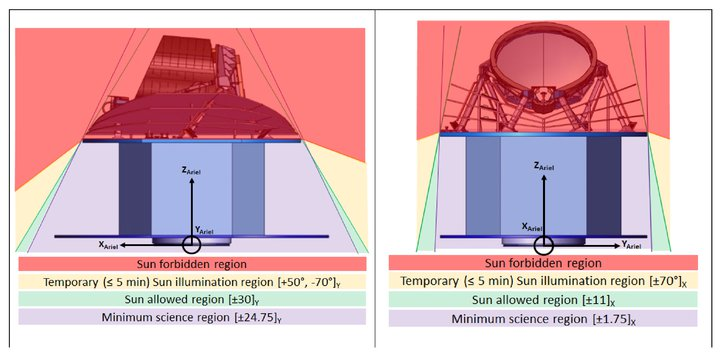
\includegraphics[width=.9\textwidth]{sun no touch.jpg}
    \caption{Illustration of the Sun allowed region (green) in the XZAriel plane (left, showing associated rotations around YAriel) and YZAriel plane (right, showing associated roatations around XAriel) \protect\cite{salvignol2024ariel}.}
    \label{fig:6}
\end{figure}

During operations, the spacecraft maintains a constrained field of regard but is capable of a full 360-degree roation around its z-axis for optimal target observations. Specific attitude control strategies around the x- and y-axes allow for extended observations of single targets without the need for spacecraft slewing \cite{salvignol2024ariel}.

\subsubsection{Attitude and Autonomy}

The nominal mission lifetime is set at four years, with a possible extension to six years based on performance and operational requirements \cite{salvignol2024ariel}. Mission operations will be conducted through two primary centres:

\begin{itemize}
    \item[-] The \textbf{Mission Operations Centre (MOC)} at ESA's European Space Operations Centre (ESOC), responsible for spacecraft operations and telemetry management \cite{salvignol2024ariel}.
    \item[-] The \textbf{Science Ground Segment (SGS)}, which includes the \textbf{Science Operations Center (SOC)} at ESA's European Space Astronomy Centre (ESAC), and the \textbf{Instrument Operations and Science Data Centre (IOSDC)}, managed by the Ariel Mission Consortium (AMC) \cite{salvignol2024ariel}
\end{itemize}

Due to limited ground station contact periods, Ariel is designed to operate autonomously for at least six days at a time. The \textbf{Attitude and Orbit Control System (AOCS)} autonomously adjusts the spacecraft's orientation to meet the pointing requirements. Attitude adjustments are pre-planned and uploaded in advance, allowing for the 6 days of autonomous operations for onboard maneuvres and payload configuration commands \cite{salvignol2024ariel}.
These adjustments are executed through ground-commanded attitudes, uplinked target quaternions, or pre-computed attitude profiles from ground control \cite{salvignol2024ariel}.
Autonomous control is crititcal for maintaining operational integrity, particularly for avoiding Sun exclusion and restricted zones (see Figure \ref{fig:6}). If the AOCS inadvertently directs the spacecraft toward an unsafe position, the onboard Fault Detection, Isolation, and Recovery (FDIR) system prevents dangerous attitudes and ensures spacecraft safety \cite{salvignol2024ariel}.

\subsection{Observation Strategy}

Variations in the measured signal from spatially unresolved observations of an exoplanet at different points in its orbit around its host star provide insights into the planet's
atmospheric spcetrum and phase-curve modulation. Since both the star and the exoplanet are observed simultaneously, the exoplanet's signal can be isolated by comparing measurements taken at different orbital positions \cite{salvignol2024ariel}.

The Ariel mission observational strategy prioritises continuous phase-curve monitoring, even when multiple orbits are needed. Observations begin and end with the secondary eclipse, which serves as a reference point for the phase-curve measurements.
To maintain precise timing, a margin of 7\% of the orbital period is included before and after the eclipse, minimising the uncertainty in eccentricity (e) to a maximum of 0.1 \cite{salvignol2024ariel}.

Three key observation types are used to analyse different aspects of the exoplanetary atmosphere:

\begin{itemize}
    \item[-] \textbf{Emission/Reflection Spectroscopy During Eclipse/Occultation:} By comparing observations taken in and out of occultation, the planet's dayside spectrum can be determined \cite{salvignol2024ariel}.
    \item[-] \textbf{Transmission Spectroscopy During Transit:} Absorption features in the exoplanet's atmosphere are measured by analysing differences between in-transit and out-of-transit measurements \cite{salvignol2024ariel}.
    \item[-] \textbf{Phase Variation Analysis:} Monitoring changes in the planet's visible hemisphere throughout its orbit reveals insights into energy redistribution and atmospheric dynamics by detecting subtle differences between observations at various orbital phases \cite{salvignol2024ariel}.
\end{itemize}

The Table \ref{tab:3} summarises known planets from the phase-curve target list, including the number of orbits required to reach a signal-to-noise ratio (SNR) greater than 10. For thermal emission,
we report the highest SNR value between the different photometric channels, assuming a Bond albedo of A$_B$ = 0.3 for planets with T$_p$ $<$ 700 K and A$_B$ = 0.1 for planets with T$_p$ $>$ 700 K \cite{salvignol2024ariel}. 
For reflected light curves, the SNR is calculated by integrating flux over the 0.5 to 1.1 $\mu$m wavelength range, assuming a geometric albedo equal to the Bond albedo. The geometric albedo represents the raio of a planet's observed brightness (as seen from the light source) to that of an idealised,
fully reflecting, diffusively scattering disc with the same cross-section \cite{salvignol2024ariel}.

\begin{table}[H]
    \centering
    \caption{The study of variability through multi-epoch phase curves will be limited to one or two selected planets, such as HD 189733b, with plans to gather three phase curves for these targets. This comprehensive approach aims to provide a deeper understanding of the atmospheric dynamics and characteristics of the observed exoplanets \protect\cite{charnay2021phasecurve}.}
    \label{tab:3}
    \resizebox{.9\textwidth}{!}{%
    \begin{tabular}{|l|c|c|c|c|}
    \hline
    \textbf{Planet} &
      \textbf{\begin{tabular}[c]{@{}c@{}}Period\\ (days)\end{tabular}} &
      \textbf{\begin{tabular}[c]{@{}c@{}}Orbits Required\\ (SNR $>$ 10)\end{tabular}} &
      \textbf{\begin{tabular}[c]{@{}c@{}}SNR\\ (Thermal Emission)\end{tabular}} &
      \textbf{\begin{tabular}[c]{@{}c@{}}SNR\\ (Reflected Light)\end{tabular}} \\ \hline
    GJ 1214b   & 1.58 & 11     & 1.0 & 0.3 \\ \hline
    K2-266b    & 0.66 & 11     & 1.1 & 0.5 \\ \hline
    55 Cnc e   & 0.74 & 10     & 0.3 & 0.3 \\ \hline
    GJ 436b    & 2.64 & 15     & 2.0 & 0.9 \\ \hline
    GJ 3470b   & 3.34 & 10     & 0.4 & 0.6 \\ \hline
    HD 189733b & 2.22 & 1 or 3 & 5.2 & 3.0 \\ \hline
    HD 209458b & 3.52 & 1 or 3 & 6.1 & 2.3 \\ \hline
    XO-6b      & 3.77 & 10     & 7.6 & 3.5 \\ \hline
    WASP-77Ab  & 1.36 & 10     & 6.1 & 3.5 \\ \hline
    KELT-7b    & 2.73 & 10     & 5.3 & 2.8 \\ \hline
    WASP-74b   & 2.14 & 9      & 7.6 & 3.4 \\ \hline
    XO-3b      & 3.19 & 9      & 5.1 & 3.5 \\ \hline
    WASP-82b   & 2.71 & 7      & 8.8 & 3.0 \\ \hline
    WASP-14b   & 2.24 & 7      & 5.1 & 2.3 \\ \hline
    KELT-O14b  & 1.71 & 7      & 1.1 & 3.9 \\ \hline
    \end{tabular}%
    }
\end{table}

\subsection{Operational Phases}

Following launch, Ariel will undergo a transfer phase of approximately 1 month before reaching the final L2 orbit. The launcher will place the spacecraft on a direct transfer trajectory, requiring three planned control maneuvres \cite{salvignol2024ariel}:

\begin{itemize}
    \item[-] The first maneuvre will occur within 1 day after separation from the launcher, but no later than 2 days.
    \item[-] No additional insertion maneuvre is required.
    \item[-] A six-month commissioning and calibration phase following launcher separation, including 1 month for transfer operations and 5 months of calibration at L2.
\end{itemize}

\begin{figure}[H]
    \centering
    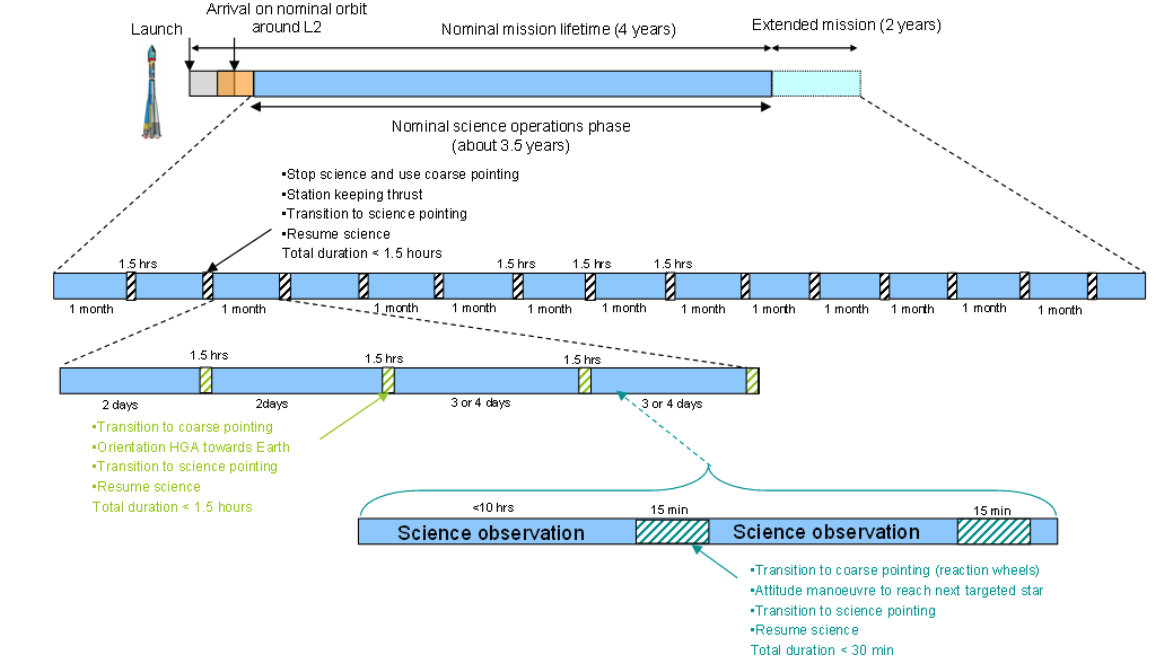
\includegraphics[width=.9\textwidth]{science interruptions.png}
    \caption{\centering Overall Science operation plan and interruptions \protect\cite{salvignol2024ariel}.}
    \label{fig:7}
\end{figure}

Once in the L2 orbit, the spacecraft maintains high availability for scientific observations with only minimal interruptions (see Figure \ref{fig:7}) \cite{salvignol2024ariel}:

\begin{itemize}
    \item[-] \textbf{Station-Keeping Maneuvres:} Conducted every 28 days, requiring less than 2 hours.
    \item[-] \textbf{Data Transmission:} Performed every 2-4 days, the spacecraft reorients its high-gain antenna toward Earth to transmit science data, requiring less than 1.5 hours.
    \item[-] \textbf{Target Transition Maneuvres:} Between successive observations, pointing adjustments and stability convergence require less than 20 minutes.
\end{itemize}

Typical Science observation slots last an average of 7.7 hours, with a maximum duration of up to 3 days per target \cite{salvignol2024ariel}.
Inaction slots are inevitable for the Ariel mission, but through simulation it has been demonstrated that 85\%-90\% of the mission lifetime is available for Science observations, including extra observations of target exoplanets, observations of backup targets,
or using the time for ancillary science (see Figure \ref{fig:8}) \cite{arielstudyreport}.

\begin{SCfigure}[50][ht]
    \centering
    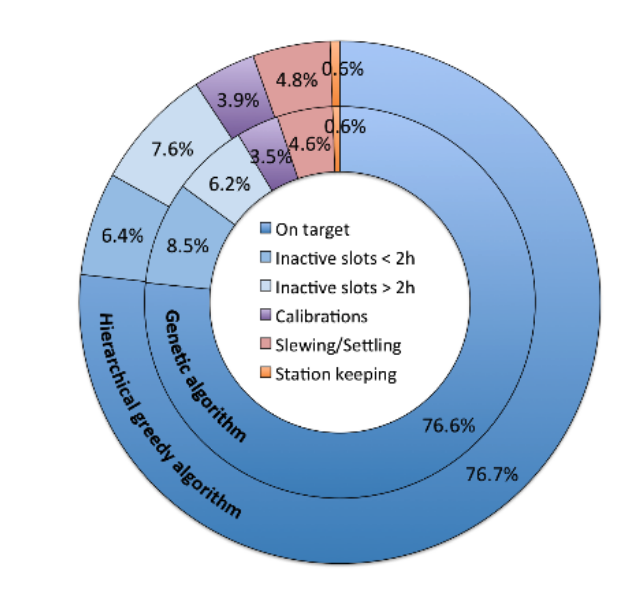
\includegraphics[width=.5\textwidth]{distribution ariel.png}
    \caption{Distribution of the mission lifetime between different operations considered in the Ariel mission planning of the MRS target list. Inner and outer ring charts correspond to the genetic and hierarchical greedy algorithms, respectively. More than
    85-90\% of the time can be used for MRS (on targets time), ancillary science targets (inactive slots), or science calibration observations \protect\cite{arielstudyreport}.}
    \label{fig:8}
\end{SCfigure}

\newpage

\section{Scientific Objectives}

\subsection{Past Exoplanet Characterisation Efforts}

Nasa's Kepler, K2, and TESS missions, alongside ESA's Cheops and PLATO, use visible light to find exoplanets by detecting their transits or measuring their sizes after discovery through radial velocity \cite{ARIEL_M4_Proposal}.
These missions have already found thousands of exoplanets, especially around bright stars, and many more will be discovered in the coming years. The next big step is measuring and studying these planets' atmospheres using infrared (IR) spectroscopy, which can reveal their chemical composition.
However, none of these missions are designed for that, most taking measurements in visible light \cite{platofact,keplerfact} \cite[p.8]{tessfact}, with Cheops the closest at near-infrared \cite[p.4]{fortier2024cheops}.
ESA's Ariel will be the first mission fully dedicated to analysing the atmospheres of hundreds of exoplanets using IR spectroscopy, helping scientists understand their makeup and temperature, expanding our knowledge of planets beyond the Solar System \cite{salvignol2024ariel,ARIEL_M4_Proposal}.

\subsection{Criteria for Exoplanet Selection}

In order for the selected sample of observed exoplanets to be statistically significant and representative, both the number of observed planets and the sample must be diverse \cite{zingales2018ariel}.
The planets must therefore be selected in accordance to various criteria; the sample must contain both gaseous and rocky planets across a range of temperatures, and the host stars must also be of
different spectral types and metallicity. A correspondingly large number of planets covering the widest possible spectrum can be sourced and selected from exoplanets discovered by previous missions, such as
the Kepler Space Mission \cite{zingales2018ariel} and the Transiting Exoplanet Survey Satellite (TESS) \cite{arielTESScandidates}.

The Ariel mission will focus primarily on planets with an orbital period that's less than 50 days, typically corresponding to warmer planets (see Figure \ref{fig:9}). 

\begin{figure}[H]
    \centering
    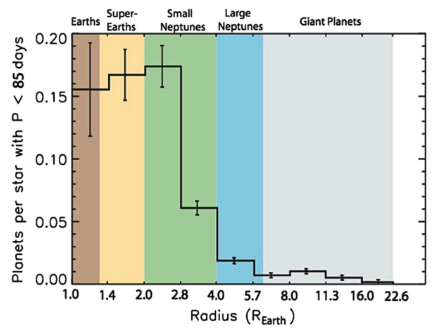
\includegraphics[width=.75\textwidth]{planet w small orbits.png}
    \caption{Average number of planets per star and per size bin with an orbital period shorter than 85 days orbiting around F, G, K stars \protect\cite{zingales2018ariel}}
    \label{fig:9}
\end{figure}

\subsection{Ariel Tier List System for Observational Prioritisation}

To maximise the science return of the Ariel mission, a three-tiered system has been devised where the three different samples are observed at optimised spectral resolutions, wavelength intervals,
and SNR \cite{salvignol2024ariel}. An additional fourth tier has been planned for additional science time to observe the pahse curves of Tier 3 planets \cite{arielstudyreport} (see Table \ref{tab:1}, Table \ref{tab:2}).

\begin{table}[H]
    \caption{Table of the Ariel tiers presented, with percentage of dedicated mission lifetime and requirements for each tier shown \protect\cite{arielstudyreport,salvignol2024ariel}.}
    \centering
    \label{tab:1}
    \resizebox{\textwidth}{!}{        
        \begin{threeparttable}
            \renewcommand{\arraystretch}{1.55}
            \begin{tabular}{|l@{\hskip 15pt}|l|}
            \hline
            Survey ($\sim$30\%)\protect\tnote{**} &
            \begin{tabular}[c]{@{}l@{}}Low spectral resolution observations (R $\geq$ 10 across all channels) of a large sample\\ of planets in the VIS-IR, with SNR $\geq$ 7\end{tabular} \\ \hline
            Deep ($\sim$60\%)\protect\tnote{**} &
            \begin{tabular}[c]{@{}l@{}}Intermediate spectral resolution observations (R $>$ 50 in AIRS channel 0 and R $>$ 15 \\ in AIRS channel 1) of a sub-sample in the VIS-IR\end{tabular} \\ \hline
            Benchmark ($\sim$6\%)\protect\tnote{**}    & Very best planets, re-observed multiple times with all techniques; full spectral resolution \\ \hline
            Phase Curves ($\sim$4\%)\protect\tnote{**} & Multiple-band photometry/spectroscopy with SNR $\geq$ 4; spatial variability                     \\ \hline
            \end{tabular}%
            \begin{tablenotes}
                \footnotesize
                \item[**] \textit{\% correspond to mission lifetime spent at each tier}
            \end{tablenotes}
        \end{threeparttable}
    }
\end{table}

\begin{table}[H]
    \caption{The total science time is $\sim$24 800 hr over the primary 4-year mission lifetime. Table of mission time required to achieve different observation goals. Note that for some bright targets (e.g. HD 209458b) Tier 2 or Tier 3 
    resolutions would be reached in a single observation \protect\cite{arielstudyreport}.}
    \centering
    \label{tab:2}
    \resizebox{.8\textwidth}{!}{%
        \begin{tabular}{lcc}
        \multicolumn{3}{c}{Mission Time Required to Achieve Different Observation Goals}                                                                       \\ \hline
        \textbf{Number of Planets} &
        \textbf{Observation Requirement} &
        \textbf{Required Science Time (hr)} \\ \hline
        1000 & Achieve Tier 1 resolutions                                                               & $\sim$10 600 \\ \hline
        \begin{tabular}[c]{@{}l@{}}400\\ \\ 500\\ 600\end{tabular} &
        \begin{tabular}[c]{@{}c@{}}Increase resolution from Tier 1\\ to Tier 2\end{tabular} &
        \begin{tabular}[c]{@{}c@{}}$\sim$3100\\ \\ $\sim$6000\\ $\sim$10 500\end{tabular} \\ \hline
        \begin{tabular}[c]{@{}l@{}}200\\ \\ 300\\ 400\end{tabular} &
        \begin{tabular}[c]{@{}c@{}}Achieve Tier 1 resolutions in the\\ second method\end{tabular} &
        \begin{tabular}[c]{@{}c@{}}$\sim$1400\\ \\ $\sim$2500\\ $\sim$4200\end{tabular} \\ \hline
        50   & \begin{tabular}[c]{@{}c@{}}Tier 3 (five repeated observations\\ per planet)\end{tabular} & $\sim$1700   \\ \hline
        ...  & Tier 4 (additional science time)                                                         & $\sim$2300   \\ \hline
        \end{tabular}%
    }
\end{table}

The orbit and attitude limits of the spacecraft must also be considered for measurements during scheduling in order to maximise the science time. Figure \ref{fig:1} illustrates the distribution of targets in right ascension and declination (equatorial) coordinates for the fraction of the year
that each region of the sky is visible within Ariel's assumed proposed orbit at the Sun-Earth Lagrangian point L2. Any direction is observable for at least $\sim$30\% of the year \cite{zingales2018ariel,morales2022ariel}.

\begin{figure}[H]
    \centering
    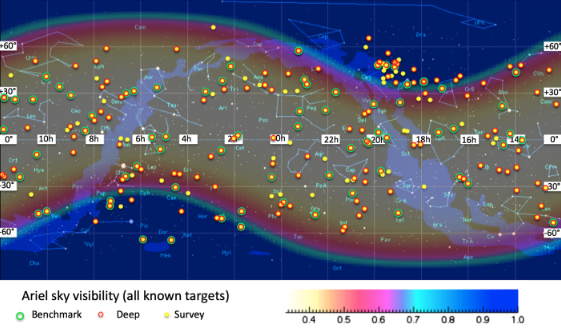
\includegraphics[width=.9\textwidth]{ariel target map.png}
    \caption{A plot illustrating the fraction of the year for which a given location in the sky (in equatorial coordinates) is visible to Ariel, as seen from a representative operational
    orbit of Ariel at L2. \textbf{Yellow} dots: planets observed in Tier 1. \textbf{Red} dots: planets observed in Tier 2. \textbf{Green} dots: planets observed in Tier 3. \protect\cite{zingales2018ariel} The background colour levels represent the fraction of the year for which
    region of the sky is visible for Ariel \cite{morales2022ariel}.}
    \label{fig:1}
\end{figure}

\subsubsection{Survey (Tier 1)}

Tier 1 observations will help refine orbital and planetary parameters that can then be used to limit or completely remove degeneracies in the interpretation of mass-radius diagrams.
Most giant planets and Neptunes fulfil the Tier 1 criteria set for the science objectives in 1 transit/eclipse, while the smaller planets would require upwards fo 6 events (see Figure \ref{fig:3}) \cite{zingales2018ariel}.
Additionally, it will be possible to generate colour-colour and colour-magnitude diagrams, which might lead to the same developments in understanding as the H-R diagram did \cite{edwards2019updated,salvignol2024ariel}.

\begin{figure}[H]
    \centering
    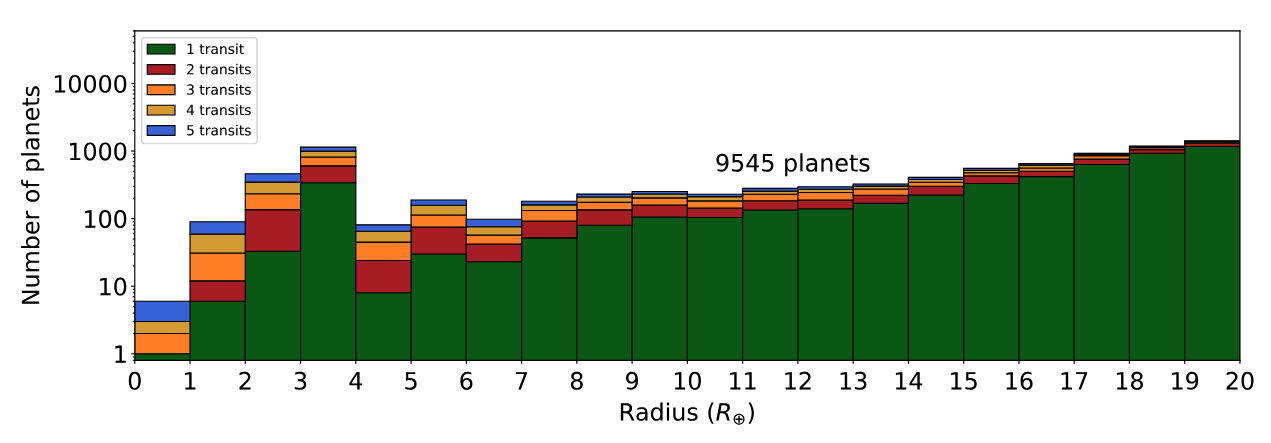
\includegraphics[width=.9\textwidth]{tier 1 transit graph.png}
    \caption{Complete set of Tier 1 planets from the Ariel mission reference population. The final list of Tier 1 planets will include an optimal sub-sample. Different colours indicate the number of transits/eclipses needed to reach
    Tier 1 performances. The planets shown here can achieve the Tier 1 requirements combining the signal of $\leq$ 5 transits/eclipses \protect\cite{zingales2018ariel}.}
    \label{fig:3}
\end{figure}

Tier 1 observations will answer the following questions:

\textbf{"What fraction of planets are covered by clouds?"}\\
This method of observation between planets with clear atmospheres and those denser cloud cover, as this obscures molecular absorption features typically present in spectra.
Extremely cloudy planets can be identified from low-resolution across a broad wavelegnth range. This assessment allows scientists to determine whether a planet should continue with higher-resolution spectral classification
(i.e., be included in the Tier 2 sample) or not \cite{salvignol2024ariel}.\\

\textbf{"What fraction of small planets still have hydrogen and helium retained from the protoplanetary disc?"}\\
This question is essential to understand the formation and evolution of super-Earths. Primordial (or primary) atmospheres are expected to be consisted of mainly hydrogen and helium,
reflecting the gaseous composition of the protoplanetary nebula. If an atmosphere is made up of heavier metals, it likely indicates that the atmosphere has evolved and thus resulting in a secondary atmosphere.
The easiest way to differentiate between primary (hydrogen-rich) and secondary (metal-rich) atmospheres is through transmission spectroscopy as the main atmospheric component directly affects the atmospheric scale height \cite{salvignol2024ariel}. \\

\textbf{"What is the bulk composition of the terrestrial exoplanets?"}\\
Planetary density provides insight into the composition of a planet's interior, but this measurement alone may lead to non-unique interpretations. Analysing the composition of the upper atmosphere in transiting planets will help reveal the degree 
of composition separation between the planet's atmosphere and interior. This approach reduces uncertainties in the presence and mass of the atmosphere, therefore resolving potential doubtfulnes in understanding the planet's overall makeup \cite{salvignol2024ariel}. \\

\textbf{"What is the energy balance of the planet?"}\\
Through analysis of eclipse measurements in optical and infrared wavelengths scientists can determing the overall temperature and albedo (the fraction of diffracted sunlight) of the planet. These measurements
help estimate the planetary energy balance and whether the planet has an internal heat source or not \cite{salvignol2024ariel}.

Ariel's Tier 1 survey mode will allow for fast and comprehensive initial assessments of planets, which allows for informed decisions when deciding what planets to further focus on during Tier 2 and Tier 3 observations \cite{salvignol2024ariel}.
Observing Figure \ref{fig:2}, illustrating the distribution of potential Tier 1 targets for the Ariel mission as functions of planetary radius and temperature, it can be seen that over 500 currently known planets already comply with the requirements for Tier 1 observations \cite{arielstudyreport,edwards2019updated}.

\begin{figure}[H]
    \centering
    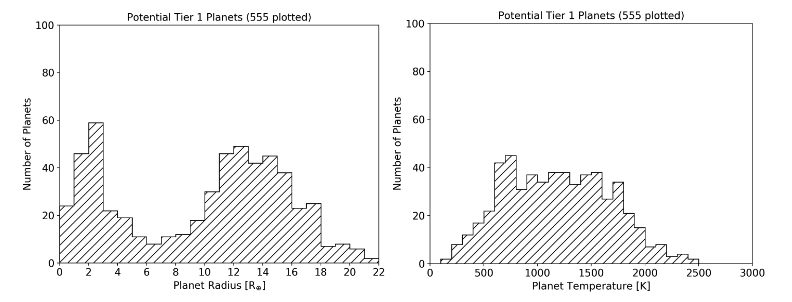
\includegraphics[width=.9\textwidth]{tier 1 radius and temp plots.png}
    \caption{Currently known Ariel planetary candidates plotted as a function of planetary radius (left) and planetary temperature (right) \protect\cite{arielstudyreport}.}
    \label{fig:2}
\end{figure}

\subsubsection{Deep (Tier 2)}

A key objective of the Ariel mission is to investigate whether a correlation exists between a planet's chemical composition and the fundamental properties such as mass, radius, and temperature. To achieve this, the Tier 2 observations will conduct high-resolution spectroscopic measurements with focus on studying both individual
exoplanets and populations. This approach allows for detailed examinations of various exoplonatery atmospheric characteristics, including \cite{salvignol2024ariel}:

\begin{itemize}
    \item[-] \textbf{Primary Atmospheric Composition in Smaller Planets:} Identifying the main gases in the atmosphere of smaller exoplanets, which is essential for characterising their atmospheric properties \cite{salvignol2024ariel}.
    \item[-] \textbf{Trace Gas Abundance:} Measuring the abundance and concentration of trace gases to determine the type of chemistry happening in the atmosphere, and whether it is in equilirbrium of non-equilibrium states \cite{salvignol2024ariel}.
    \item[-] \textbf{Atmospheric Thermal Structure:} Analysing the thermal structure, both vertically and horizontally, of the atmosphere to understand the impact on atmospheric structure and energy distribution \cite{salvignol2024ariel}.
    \item[-] \textbf{Cloud Characteristics:} Examining cloud properties, such as particle size and distribution, to understand their impact on climate and atmospheric dynamics \cite{salvignol2024ariel}.
    \item[-] \textbf{Elemental Composition in Gaseous Planets:} Investigating the elemental makeup of gaseous planets to constrain formation models and enhance the understanding of planetary evolution \cite{salvignol2024ariel}.
\end{itemize}

By integrating these measurements, the Tier 2 Deep Survey observations aim to provide a comprehensive view and understanding of atmospheric characteristics in a broad range of exoplanets, enabling comparisons across different planetary populations and contributing to the advancement of the broader goals of the Ariel mission \cite{salvignol2024ariel}.

\subsubsection{Benchmark (Tier 3)}

The Ariel Tier 3 observations are dedicated to the detailed study of atmospheric variability in a select group of exoplanets, known as benchmark planets. A portion of these planets, particularly those obiting very bright stars, will be observed multiple times over an extended period of time to gather essential data. The key objectives of these observations include \cite{salvignol2024ariel}:

\begin{itemize}
    \item[-] \textbf{Primary Knowledge of Planetary Chemistry and Dynamics:} Examining the chemical processes within exoplanet atmospheres to better understand their composition and behaviour \cite{salvignol2024ariel}.
    \item[-] \textbf{Elemental Composition Analysis:} Investigating the distribution of elements, both within the atmosphere and on the planet's surface, to gain insights into formation and evolutionary history \cite{salvignol2024ariel}.
    \item[-] \textbf{Weather Patterns and Atmospheric Variability:} tracking spatial and temporal changes in atmospheric conditions, including temperature variations, cloud coverage, and atmospheric circulation dynamics, to gain insight into the weather systems of exoplanets \cite{salvignol2024ariel}.
\end{itemize}

Benchmark planets are identified as ideal candidates for phase-curve spectroscopic measurements due to their high spectral resolution and strong signal-to-noise ratios (SNR), allowing for meaningful observations in just one or two observations.
The focus will be on "weather planets", selected for their potential to showcase significant atmospheric changes over time \cite{salvignol2024ariel}.

By conducting repeated observations, Ariel Tier 3 observations aim to capture the temporal evolution of exoplanetary atmospheres, revealing essential insights into cloud formation, atmospheric circulation, and climate dynamics on exoplanets \cite{salvignol2024ariel}.
Figure \ref{fig:4} shows a possible MRS (Mission Reference Sample) with all the three tiers discuss (Survey, Deep, Benchmark) nested together, optimised to yield maximum number of targets. 

\begin{figure}[H]
    \centering
    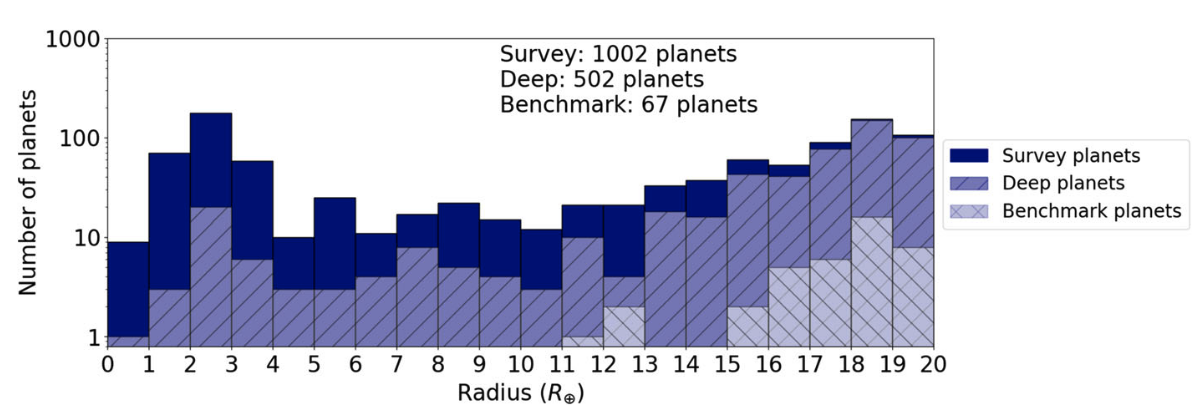
\includegraphics[width=.9\textwidth]{comparison tiers.png}
    \caption{Overview of the Ariel MRS (Mission Reference Sample), comparing the number of planets observable in the three tiers during the mission lifetime \protect\cite{zingales2018ariel}.}
    \label{fig:4}
\end{figure}

\subsubsection{Phase Curves (Tier 4)}

To gain deeper insights on targets of special interest, bespoke observations are conducted to study their spatial variability and gather detailed information on planetary chemistry and atmospheric dynamics. 
Tier 4 planets will be selected from Tier 3 Benchmark planets based on their potential to exhibit significant atmospheric variability (see Figure \ref{fig:5}) \cite{edwards2022ariel}.
A key method used in analysis is through observing planetary phase curves, which answers several fundamental questions \cite{arielstudyreport}:

\begin{itemize}
    \item[-] \textbf{Factors Influencing Atmospheric Heat Redistribution:} This investigation aims to identify how factors such as stellar irradiation, planetary radius, metallicity (the abundance of elements heavier than hydrogen and helium), and orbital eccentricity
    impact the atmospheric heat redistribution. By measuring dayside and nightside emissions, as well as phase offsets, researchers can gain details about circulation regimes, radiative timescales, wind speeds, and the role of nightside clouds \cite{arielstudyreport}.
    \item[-] \textbf{Variations in Atmospheric Composition and Thermal Structure:} This analysis focuses on how the chemical composition and thermal structure of strongly irradiated planets change from the dayside to the nightside. Atmospheric circulation is expected to smooth
    out variations, leading to chemical disequilibrium, and potential temperature fluctuations and thermal variations on the dayside \cite{arielstudyreport}.
    \item[-] \textbf{Atmospheric Composition of Low-Mass Planets:} A key objective is determining the atmospheric composition and metallicity of low-mass exoplanets. It is predicted that planets with higher atmospheric metallicity will exhibit greater heat redistribution and higher
    amplitude phase curves, allowing or independent measurements of atmospheric metallicity \cite{arielstudyreport}.
    \item[-] \textbf{Albedo of Exoplanets:} This question investigates the nature of tiny particles present in exoplanetary atmospheres, particularly condensate clouds and photochemical hazes. Measuring the planet's albedo is important for understanding its temperature balance.
    Since temperature variations can influence the albedo, understanding this relationship can provide valuable insights into exoplanet climate and atmospheric conditions \cite{arielstudyreport}.
\end{itemize}

By integrating these observations, researchers can develop a more comprehensive understanding of exoplanetary atmospheres, their dynamic, chemistry, and climate, further advancing the field of comparative planetology.

\begin{SCfigure}[50][hb]
    \centering
    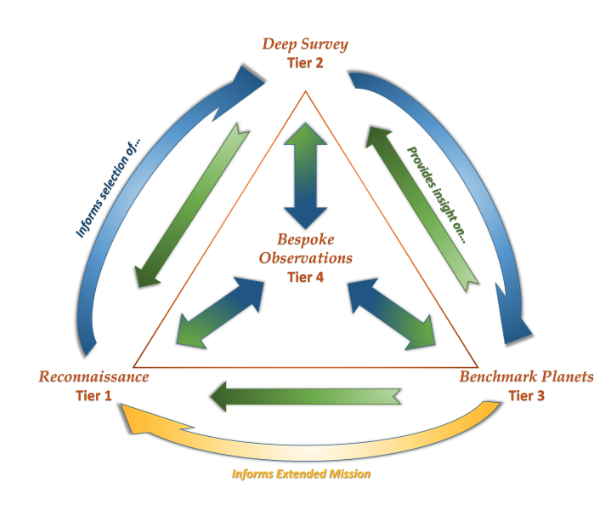
\includegraphics[width=.55\textwidth]{tiers ariel.png}
    \caption{Schematic diagram of Ariel's 4-Tier ecosystem. Tier 1 will provide the base for selecting Tier 2 planets, which in turn inform the selection of Tier 3 targets. The planets in each Tier will give us deeper insight into the nature of the planets in preceding Tiers. This interdependence among Tiers means that the
    scientific value of the data collected by Ariel will grow over time. Tier 4 observations will benefit from the insight gained by the planetary populations of the other Tiers and will in turn provide a better understanding of their atmospheric behaviour \protect\cite[p.40]{arielstudyreport}.}
    \label{fig:5}
\end{SCfigure}

\subsection{The Scientific Reasoning for Studying Hot Exoplanets}

Hot planets provide a unique opportunity to study their elemental and chemical composition because their atmospheres lack cold traps that would otherwise condense key molecules, like H$_2$O NH$_3$, CH$_4$, SiO, CO$_2$, CO, and, at high temperatures, metallic compounds such as TiO, VO, and CrH \cite{ARIEL_M4_Proposal} \cite[p.135]{tinetti2018chemical}.
Understanding these hot planets is crucial for building a broad foundation before shifting the focus to cooler planets. Moreover, many of the exoplanets discovered so far, or expected to be found, are in close orbits around their stars, making them naturally hot. Their short orbital periods make them ideal candidates for transit and eclipse spectroscopy, allowing detailed
atmospheric studies. While the ultimate goal is to characterise a wide range of exoplanets, including potentially habitable ones, Ariel will serve as a crucial stepping stone, paving the way for even more advanced future missions \cite{ARIEL_M4_Proposal}.

\subsection{Expected Discoveries}



\newpage

\section{Spacecraft Overview}

\subsection{General Spacecraft Design}


\subsubsection{Key Components and Subsystems}


\subsection{Service Module (SVM)}


\subsection{Payload Module (PLM)}

\subsubsection{Ariel IR Spectrometer (AIRS)} 

\subsubsection{Fine Guidance System (FGS)}

\subsubsection{Analysis and Testing of the PLM}

\paragraph{Surface Charging Analysis} ~\\
filler

\paragraph{Thermoelastic Analysis} ~\\
filler


\newpage

\section{Conclusion}

\newpage

%%%%%%%%%%%%%%%%%%%%%%%%%%%%%%%%%%%

\bibliographystyle{IEEEtran}
\bibliography{References} \label{sec:ref}

\vspace{1.5cm}

\section*{Contributions}
\addcontentsline{toc}{section}{Contributions}

\subsection*{Joana Carranço Cabral Adão}


\subsection*{Kyla Boyle}


\subsection*{Ewan Finlayson}


\subsection*{Ananya Laxmeshwar}


\subsection*{Isha Mathew}


\subsection*{Matilda Onnebrink}


\subsection*{Brian Woods}


\listoffigures

\listoftables

\section*{Appendix}
\addcontentsline{toc}{section}{Appendix}


\end{document}